
\subsubsection{Definitionen für ungerichtete Graphen}

Ungerichteter Graph $G=(V,\; E)$\\
Knotenmenge $V=V(G)$\\
Kantenmenge $E=E(G)$\\
Relation $E \rightarrow V \times V$\\
\hspace{8mm} $e=\{u,\; v\}$\\
"`e ist inzident mit $u$ und $v$ "'\\
"`$u$ und $v$ sind adjazent"'\\

\begin{tabular}{c@{\hspace{5mm}}c}
parallele Kanten&Schleife\\
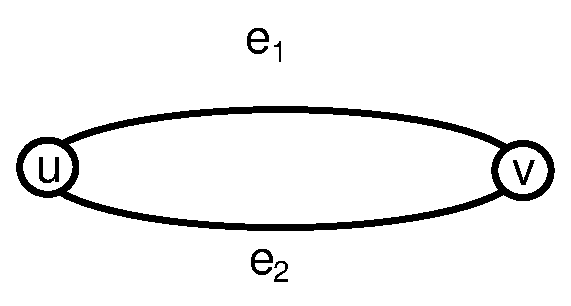
\includegraphics[width=4cm]{bilder/2-0ParalleleK}&
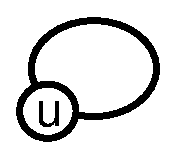
\includegraphics[width=1cm]{bilder/2-0Schleife}
\end{tabular}

Einfacher Graph: \begin{itemize}\item keine parallelen Kanten
\item keine Schleifen\end{itemize} 

"`$e=u v$"' \hspace{10mm} "`$e = v u$"'

Subgraph $H$ von $G$
\begin{itemize}
\item[\mbox{}] $V(H) \subseteq V(G)$
\item[\mbox{}] $E(H) \subseteq E(G)$
\end{itemize}

$A \subseteq E$ \hspace{2mm} $G\wout A$: Subgraph von $G$ nach Entfernen der Kanten in $A$ 

$B \subseteq V$ \hspace{2mm} $G \wout B$: Subgraph von G nach
entfernen der Knoten in $B$ und aller inzidenter Kanten. Kann auch als
$G(V\wout B)$ oder als durch $V \wout B $ indizierter Subgraph
bezeichnet werden. 

"`$G \wout x$"' statt $G \wout \{x\}$ für $x \in V$ oder $x \in
E$\\

$n=|V|$ \hspace{4mm} $m = |E|$ \hspace{4mm} Konvention\\

Ein Subgraph $H$ von $G$ ist aufspannend\\
$\Leftrightarrow V (H) = V$\\

Weg $P$ in $G$: Folge $\begin{array}[t]{l}
v_{0}, e_{1}, v_{1}, \ldots, e_{k}, v_{k}\\
v_{0}, v_{1}, \ldots, v_{k} \in V, \hspace{3mm} e_{1}, e_{2}, \ldots, e_{k}
\in E\\
e_{i} = v_{i-1} v_{i} \; \; \; \mbox{für}\; \;  1 \leqq i \leqq k
\end{array}$

"`Weg von $v_{0}$ nach $v_{k}$"' oder "`$(v_{0}, v_{k})$-Weg"'\\
Der Weg ist geschlossen, falls $v_{0} = v_{k}$\\
Der Weg ist einfach, falls $v_{0}, v_{1}, \ldots, v_{k}$ distinkt\\
Ein Weg ist ein Kreis falls:
\begin{enumerate}
\item Geschlossenheit
\item $v_{0}, v_{1}, \ldots, v_{k}$ distinkt sind
\item $k \geqq 1$
\end{enumerate}

$G$ hat $(u,v)$-Weg $\Rightarrow$ $G$ hat einen einfachen $(u,v)$-Weg\\
Länge von $P= v_{0}, e_{1}, v_{1}, \ldots, e_{k}, v_{k}$: $k$

$G$ ist zusammenhängend :$\Leftrightarrow$ zu jedem Knotenpaar $(u,v)$ aus $V$
gibt es einen $(u,v)$-Weg

\section{Minimal aufspanndende Bäume} 

Beispiel:


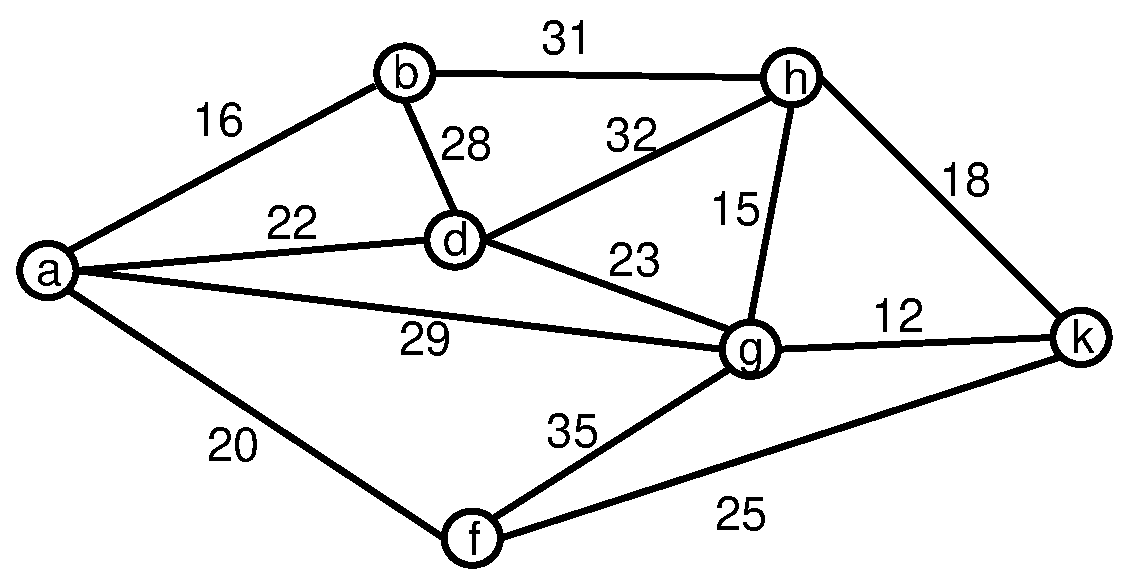
\includegraphics[width=10cm]{bilder/2-1NetzwerkP}

Dieses Netzwerk sei ein Kommunikationsnetzwerk und bilde Terminals ab und 
die den Kanten zugeordneten Zahlen entsprächen den Kosten für die direkte 
Verbindung zwischen den Terminals damit ergibt sich das

\subsubsection{Verbindungs-Problem}

Gegeben: Ein zusammenhängender Graph $G=(V,E)$ und positive Kosten für alle
$e \in E$\\
Gesucht: Ein aufspannender, zusammenhängender Subgraph mit minimalen
Kosten.

\begin{lemma}
Eine Kante $e=u v \in E$ ist Kante eines Kreises in $G$ genau dann, wenn es
einen $(u,v)$-Weg in $G \wout e$ gibt.
\end{lemma}

$\rightarrow$ die Optimallösung des Verbindungs-Problems hat keine Kreise

Einen Graphen ohne Kreis nennt man auch Wald, einen zusammenhängenden Wald
nennt man auch Baum.

\subsubsection{Minimal aufspannendes Baum-Problem}

Gegeben: Ein zusammenhängender Graph $G(V,E)$ $c_{e} \in R$ für alle $e 
\in E$\\
Gesucht: Der Aufspannende Baum in G mit minimalen Kosten (MSB) im
Englischen (MST = minimal spanning tree). Das Verbindungs-Problem und das
MSB-Problem sind äquivalent für $c_{e} > 0$.

Nun ein bisschen Wiederholung aus Informatik I:\\
Notation: $G = (V,E)$\\
$A \subseteq V$: $\delta(A) := \{u v \in E| \underbrace{u \in A,\; v\in
V \wout A}_{\mbox{\scriptsize Kanten die auf den Schnitten liegen}}\}$\\
$\delta(A)$ wird auch als "`Schnitt in G"' bezeichnet (indiziert von $A
\subseteq V$)\\ 
$\gamma(A) = \{u,v \in A, \; \; u v \in E\}$ ergibt alle Kanten in $A$

\subsubsection{Prims Algorithmus für MSB}

\begin{algorithmic}
\STATE Initialisiere $H=\left(V(H),T\right)$ als $\left\{\{r\},
\varnothing\right\}$
\WHILE{(H ist nicht aufspannender Baum)}

\STATE Füge eine Kante minimaler Kosten aus $\delta\left(V(H)\right)$ zu $H$
\ENDWHILE
\end{algorithmic}

In unserem Kommunikationsproblem erhält man nun, wenn man bei Knoten a 
anfängt:

\begin{tabular}{|c|r|}
\hline
{\bf Hinzugefügte Kante}& {\bf Kosten}\\
\hline
(a, b)& 16\\
\hline
(a, f)& 20\\
\hline
(a, d)&22\\
\hline
(d, g)&23\\
\hline
(g, k)&12\\
\hline
(g, h)&15\\
\hline
\end{tabular}

\subsubsection{Kruskals Algorithmus für MSB}

\begin{algorithmic}
\STATE Sortiere E als $<e_{1}, e_{2}, \ldots, e_{m}>$, so dass $c_{e_{1}} \leqq
c_{2} \leqq \ldots \leqq c_{e_{m}}$
\STATE Initialisiere $H=(V,T)$ als $(V, \varnothing)$
\FOR{ $i = 1$ to $m$} 
\STATE {\bf if} Endknoten von $e_{i}$ in verschiedenen Komponenten von $H$
{\bf Then} Füge
$e_{i}$ zu T hinzu.
\ENDFOR
\end{algorithmic}


mit unserem Beispiel erhält man:

\begin{tabular}{|c|r|}
\hline
{\bf Hinzugefügte Kante}& {\bf Kosten}\\
\hline
(g, k)& 12\\
\hline
(g, h)& 15\\
\hline
(a, b)&16\\
\hline
(a, f)&20\\
\hline
(a, d)&22\\
\hline
(d, f)&23\\
\hline
\end{tabular}

Beide Algorithmen können mit einer Laufzeit $O(m \log n)$ implementiert
werden.

Hier legte Prof. Jünger eine Folie auf mit Punkten um die herum ein
Analogrechner Kreise "`auf bläst"' bis zwei Kreise aneinander stoßen. Wenn
zwei Kreise aneinander stoßen und zwischen den Komponenten noch keine
Verbindung besteht so wird eine Kante dort eingefügt. Mag es jemand malen?

\subsubsection{MSB und lineare Optimierung}

Notation: Menge $\begin{array}[t]{l} A, \; p \in \RR^{A}, \; \; B \subseteq A\\
p(B) = \displaystyle \sum_{j \in B} p_{j}
\end{array}$

LPMSB $\begin{array}[t]{rcl} \min c^{T}x\\
x \left(\gamma(S)\right) &\leqq& |S| -1 \; \; \; \forall S, \varnothing \not=
S \subset V\\
x(E) &=& |V| -1\\
x_{e} &\geqq& 0 \; \; \forall e \in E
\end{array}$

In diesem Fall wird explizit nicht $x_{e} \in \{0,1\}$ gefordert, da die
Ganzzahligkeits-Bedingung das Problem sehr schwer werden lässt.

Die Inzidenzvektoren $x^{0}$ von aufspannenden Bäumen T sind zulässige
Lösungen und $c^{T}x^{0} = c(T) $, d.h. gleicher Zielfunktionswert.\\
$\Rightarrow$ der Wert von (LPMSB) ist eine untere Schranke für die Kosten
eines MSB.

\begin{satz}
Sei $x^{0}$ der Inzidenzvektor eines MSB bezüglich der Kosten $c_{e}$. Dann
ist $x^{0}$ eine Optimallösung von LPMSB.\\
Beweis: Für eine Kanten-Teilmenge $A \subseteq E$ sei $\kappa(A)$ die Anzahl
der Zusammenhangs-Komponenten des Subgraphen $(V,A)$ von $G=(V,E)$:

\[\begin{array}{rcl}
\mbox{(LPMSB')} \hspace{7mm} \min c^{T}x\\
x(A) &\leqq & |V| - \kappa(A) \; \; \forall A \subset E\\
x(E) &=& |V| -1\\
x_{e} &\geqq& 0 \; \; \forall e \in E
\end{array}\]
\end{satz}

Beweis: Das (LPMSB') hat die gleiche zulässigen Lösungen wie das (LPMSB)
d.h. auch die gleiche Optimallösung. In $x(A) \leqq |V| - \kappa (A)$
setzen wir speziell $A = \gamma(S)$ und erhalten:

\[\begin{array}{rcl}
x\left(\gamma(S)\right) &\leqq & |V| - \underbrace{\kappa\left(\gamma(S)
\right)}_{\geqq | V \wout S| + 1}\\
&\leqq& |V|-| V \wout S | -1\\
&=& | S | -1
\end{array}\]

Umgekehrt folgt $x(A) \leqq |V| - \kappa(A)$, denn:\\
Sei $A \subseteq E $ und $s_{1}, s_{2}, \ldots, s_{k} \; \left(k = \kappa(A)
\right)$ die Knotenmengen der Zusammenhangs-Komponenten von $(V,A)$.\\
Dann gilt $\begin{array}[t]{rcl} 
x(A) &\leqq & \displaystyle \sum_{i=1}^{k} x\left(\gamma (s_{i})\right)\\
&\leqq & \displaystyle \sum_{i=1}^{k} (|s_{i}| -1)\\
&=& |V|-k
\end{array}$

Es reicht also zu zeigen $x^{0}$ ist optimal für (LPMSB'). Wir zeigen dies
nun für ein $x^{0}$ das Ergebnis aus Kruskals Algorithmus ist. Im (LPMSB')
können wir für die Zielfunktion auch schreiben $\-max -c^{T}x$. Damit
erhalten wir als duales LP:
\[
\begin{array}{rcl}
\mbox{(DLPMSB')} \hspace{7mm} \min \displaystyle \sum_{A \subset E \mbox{\scriptsize so 
dass } e \in A} (|V| - \kappa(A)) y_{A}\\
 \displaystyle \sum_{A \subset E \mbox{ \scriptsize so dass }
e \in A} y_{A} &\geqq& -c_{e} \; \; \forall e \in E\\
y_{A} &\geqq& 0 \; \; \forall A \subset E
\end{array}
\]
$y_{E}$ ist in diesem Fall nicht vorzeichen-beschränkt. Mittels Kruskals
Algorithmus konstruieren wir nun eine Optimallösung von (DLPMSB').

Sei $e_{1}, e_{2}, \ldots, e_{m}$ die sortierte Folge der Kanten in
Kruskals Algorithmus.
\[ R_{i} := \{ e_{1}, e_{2}, \ldots, e_{i}\} \hspace{3mm} (1 \leqq i \leqq
m) \hspace{3mm} R_{0} := \varnothing \]
Weiterhin definieren wir $y^{0}$:
\[\begin{array}{rcl}
y^{0}_{R_{i}} &=& c_{e_{i+1}} - c_{e_{i}}\\
y^{0}_{R_{m}} &=& -c_{e_{m}} \hspace{3mm} \\ \hspace{3mm} y_{A}^{0} = 0 
\mbox{ sonst } \hspace{3mm} (A \not=R_{i})
\end{array}\]
Es gilt nun (wg. Sortierung) $y_{A}^{0} \geqq 0 \hspace{3mm} \forall
A \not= E$ und mit $e=e_{i}$:
\[\begin{array}{rcl}
\displaystyle \sum_{A \subset E \mbox{\scriptsize  so 
dass } e \in A} y^{0}_{A} &=& \displaystyle \sum^{m}_{j=1} y^{0}_{R_{j}} =
\sum^{m-1}_{j=i} (c_{e_{j+1}} - c_{e_{j}}) - c_{e_{m}}\\
&=& c_{e_{i+1}} - c_{e_{i}} + c_{e_{i+2}} -  c_{e_{i+1}} + \ldots
+  c_{e_{m}} -  c_{e_{m-1}} - c_{e_{m}}\\
&=& -c_{e_ {i}} = - c_{e} \end{array}
\]

$\Rightarrow$ alle "`$\geqq$"' sind mit "`="' erfüllt.\\
$\Rightarrow \left\{ \begin{array}{l}y^{0} \mbox{ ist zulässig für
(DLPMSB')}\\
\mbox{kompl. Schlupf $x_{e}^{0} > 0 \Rightarrow \displaystyle \sum_{A
\subset E \mbox{ so dass } e \in A} y_{A} = -c_{e} \; \; \forall e \in E$}
\end{array}\right.$

Noch zu zeigen:
\[\mbox{Kompl. Schlupf: } y_{A}^{0} > 0 \Rightarrow x^{0}(A) = | V | -
\kappa(A)\]
Sei $y_{A} > 0 \Rightarrow A = R_{i}$ für $1\leqq i \leqq m$\\
Annahme: $x^{0} (R_{i}) < |V| - \kappa(R_{i})$\\
$x^{0} (R_{0}) = |V| - \kappa(R_{0})$ 
$\Rightarrow \exists e \in R_{i}$: Hinzufügen von $e$ zu $T \cap R_{i}$
erniedrigt die Zahl der Zusammenhangs-Komponenten von $(V,R_{i} \cap T)$\\
$\Rightarrow e \not \in T \hspace{3mm} \lightning$ denn Kruskal hätte $e$
gewählt, d.h. $e \in T$

Damit ergibt sich nun insgesamt: $x^{0},\;y^{0}$ sind zulässig und erfüllen
die komplementären Schlupfbedingungen.\\
$\Rightarrow x^{0}$ ist optimal für (LPMSB')\\
$\Rightarrow x^{0}$ ist optimal für (LPMSB)

Bemerkung: Dies beweist die Korrektheit von Kruskals Algorithmus.

\section{Kürzeste Wege}
Anwendung: Kürzeste Fahrstrecke von A nach B in einem Straßen-Netzwerk.\\
Es gibt auch Einbahnstraßen $\rightarrow$ gerichtete Graphen\\
Gerichteter Graph $G=(V,E)$ auch genannt "`Digraph"' mit \\
$V=V(G)$ Knoten \\
$E(G)$ gerichtete Kanten oder auch Bögen (arc)\\
\begin{tabular}{ll}
Für $e \in E$:& $t(e)$: Ende von $e$ (tail)\\
&$h(e)$: Spitze von $e$ (head)
\end{tabular}
 
Die anderen Begriffe gelten analog zu nicht gerichteten Graphen.\\
Den zu einem gerichteten Graphen zugeordneten ungerichteten Graphen erhält
man durch das weglassen der Richtung.\\
Parallele Kanten sind Kanten die dieselbe Spitze und und die gleichen
Enden haben. Antiparrallele Kanten sind zwei Kanten bei denen die eine dort
die Spitze hat wo die andere das Ende und umgekehrt.

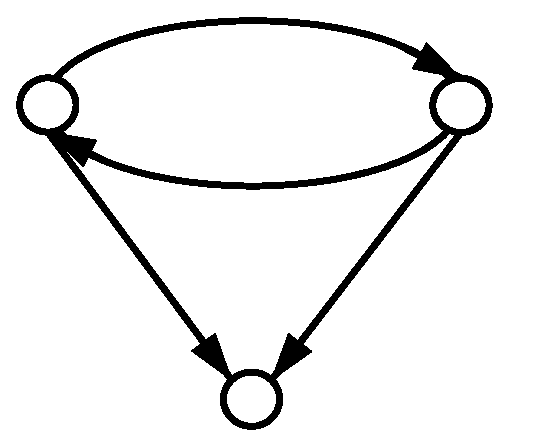
\includegraphics[height=3cm]{bilder/2-2einfachnichte} 

Als Digraph ist dieser Graph ein einfacher Graph als ungerichteter Graph
nicht.

$e=u v \rightarrow t(e)=u$, $h(e) = v$

Kanten $e_{i}$ eines Weges $P= v_{0}, e_{1}, v_{1}, e_{2}, \ldots e_{k},
v_{k}$. Der Weg heißt vorwärts gerichtet falls $t(e_{i})=v_{i-1}$ und
$h(e_{i})=v_{i}$. Analog ist ein gerichteter Kreis ein Kreis bei dem alle
Kanten vorwärts gerichtet sind.

\subsubsection{Kürzeste Wege Problem}
Gegeben: Digraph $G$, Knoten $v$ aus $V$, Gewichte $c_{e} \in \RR \; \forall 
e \in E$ 

Gesucht: Für alle $v \in V$ einen gerichteten Weg von $r$ nach $v$ mit
minimalen Kosten, falls ein solcher existiert.

Konvention: Zur Vermeidung der Nicht-Existenz eines $(r,v)$-Weges fügt man
Kanten $r v \in E$ mit sehr hohem Gewicht hinzu.

Ohne Beschränkung der Allgemeinheit kann von einem einfachen Graphen
ausgegangen werden, da man alle parallelen Kanten auf die günstigste Kante
reduziert.

Die Grundidee der folgenden Algorithmen sieht dabei folgendermaßen aus:
\begin{itemize}
\item $\forall v  \in V$ gerichteter Weg von $r$ nach $v$ mit Kosten 
$y_{v}$
\item Finde eine Kante $v w \in E$ mit $y_{v} + c_{v w} < y_{w}$: dann existiert ein
kürzester Weg (in Bezug auf alle Wege die wir bisher kennen) von $v$ nach
$w$ mit Kosten $y_{v} + c_{v w}$. 
\item Sind die $y_{v}\;\; (v \in V)$ Kosten für kürzeste $(u,v)$-Wege so 
gilt:\\ ($\ast$) $y_{v} + c_{v w} \geqq y_{w}$\\
$y \in R^{v}$ heißt zul. Potential falls  ($\ast$) gilt und $y_{r}=0$
Falls $y_{r} \not= 0$, einfach $y_{v}$ durch $y_{v} - y_{r}$ ersetzen.  
\end{itemize}

\begin{lemma} \label{Potential}
Sei $y$ ein zulässiges Potential und $P$ ein $(r,v)$-Weg (gerichtet), dann
gilt: $c(P) \geqq y_{v}$\\
\end{lemma}

Beweis: Sei $P= v_{0}, e_{1}, v_{1}, e_{2}, \ldots e_{k}, v_{k}$, mit $v_{0} 
= r$, $v_{k}=v$ so gilt:
\[c(P) = \sum^{k}_{i=1} c_{e_{i}} \geqq \sum^{k}_{i=1}(y_{v_{i}} -
y_{v_{i-1}}) = y_{v_{k}} - \underbrace{y_{v_{0}}}_{=0} = y_{v_{k}} 
\hspace{3mm} \mbox{q.e.d}\]

\begin{lemma}
Es existiert eine Lösung des Kürzeste Wege Problems, die nur Kanten eines
aufspannenden Baumes enthält
\end{lemma}

Beweis: Subwege von kürzesten Wegen sind kürzeste Wege\\
$\Rightarrow \forall v \in V, \; \; v \not=r$ genügt die letzte Kante
eines gerichteten $(r,v)$-Weges

\subsubsection{Fords Algorithmus}

\begin{algorithmic}
\STATE Initialisiere:\\
$y_{r} := 0, \; \; y_{v} := \infty \; \; \forall v \not= r$\\
$p_{r} := 0, \; \; p_{v} := -1 \; \; \forall v \not= r\; \; \; (0,-1) \not
\in V$
\WHILE{($y$ kein zul. Potential)}
\STATE Finde eine Kante $v w$ mit $y_{v} + c_{v w} < y_{w}$
\STATE setze $y_{w} := y_{v} + c_{v w}$ und $p_{w} := v$
\ENDWHILE
\end{algorithmic}

\subsubsection{Beispiel 1}

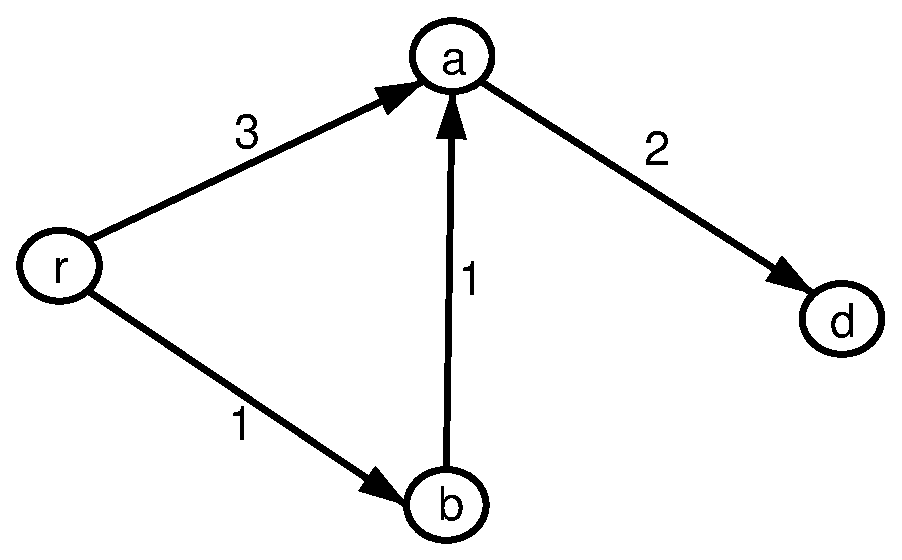
\includegraphics[width=6cm]{bilder/2-2FordBsp1}

\begin{tabular}{l|r|r|r|r|r|r|r|r|r|r|}
&\multicolumn{2}{|c|}{Start}&\multicolumn{2}{|c|}{$v w=r a$}&
\multicolumn{2}{|c|}{$v w=r b$}&\multicolumn{2}{|c|}{$v w=ad$}&
\multicolumn{2}{|c|}{$v w=a b$}\\ \hline
&y&p&\hspace{2mm}$\;$y&p&\hspace{2mm}$\;$y&p&\hspace{2mm}$\;$y&p&
\hspace{2mm}$\;$y&p\\ \hline
r&0&0&&&&&&&&\\
a&$\infty$&-1&3&$r$&&&&&2&$b$\\ 
b&$\infty$&-1&&&1&$r$&&&&\\
d&$\infty$&-1&&&&&5&$a$&4&$a$
\end{tabular}

Eigenschaften
\begin{enumerate}
\item Nach jeder Iteration gilt:
\[y_{v} \geqq y_{p(v)} + c_{p(v)v}\]
Dies gilt mit "`="' wenn $y_{v}$ und $p(v)$ gesetzt werden, nachher kann
$y_{p(v)}$ nur kleiner werden.
\item Nach Terminierung gilt:
\[y_{v} \geqq y_{p(v)} + c_{p(v)v}\]
\end{enumerate}

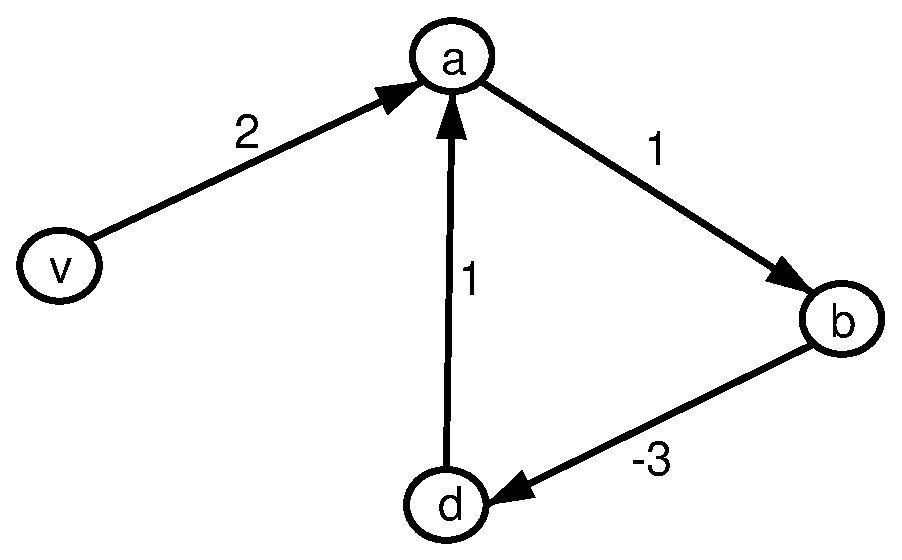
\includegraphics[width=6cm]{bilder/2-2FordBsp2}

\begin{tabular}[c]{l|r|r|r|r|r|r|r|r|r|r|r|r}
&\multicolumn{2}{|c|}{Start}&\multicolumn{2}{|c|}{$v w=r a$}&
\multicolumn{2}{|c|}{$v w=ab$}&\multicolumn{2}{|c|}{$v w=b d$}&
\multicolumn{2}{|c|}{$v w=da$}&\multicolumn{2}{|c}{$v w=ab$}\\ \hline
&y&p&\hspace{2mm}$\;$y&p&\hspace{2mm}$\;$y&p&\hspace{2mm}$\;$y&p&
\hspace{2mm}$\;$y&p&\hspace{2mm}$\;$y&p\\ \hline
r&0&0&&&&&&&&&&\\
a&$\infty$&-1&2&$r$&&&&&1&$d$&&\\
b&$\infty$&-1&&&3&$a$&&&&&2&$a$\\
d&$\infty$&-1&&&&&0&$b$&&&&
\end{tabular} $\ldots$

Hier terminiert das Verfahren nicht, da $y_{a}, \; y_{b}, \; y_{c}, \;
\rightarrow - \infty$.\\
Grund: negativer Kreis $a b d$.

Der Algorithmus soll dies erkennen. Es gibt aber auch Anwendungen für
negative Kreise, z.B. im Währungstausch.

\begin{tabular}{c}
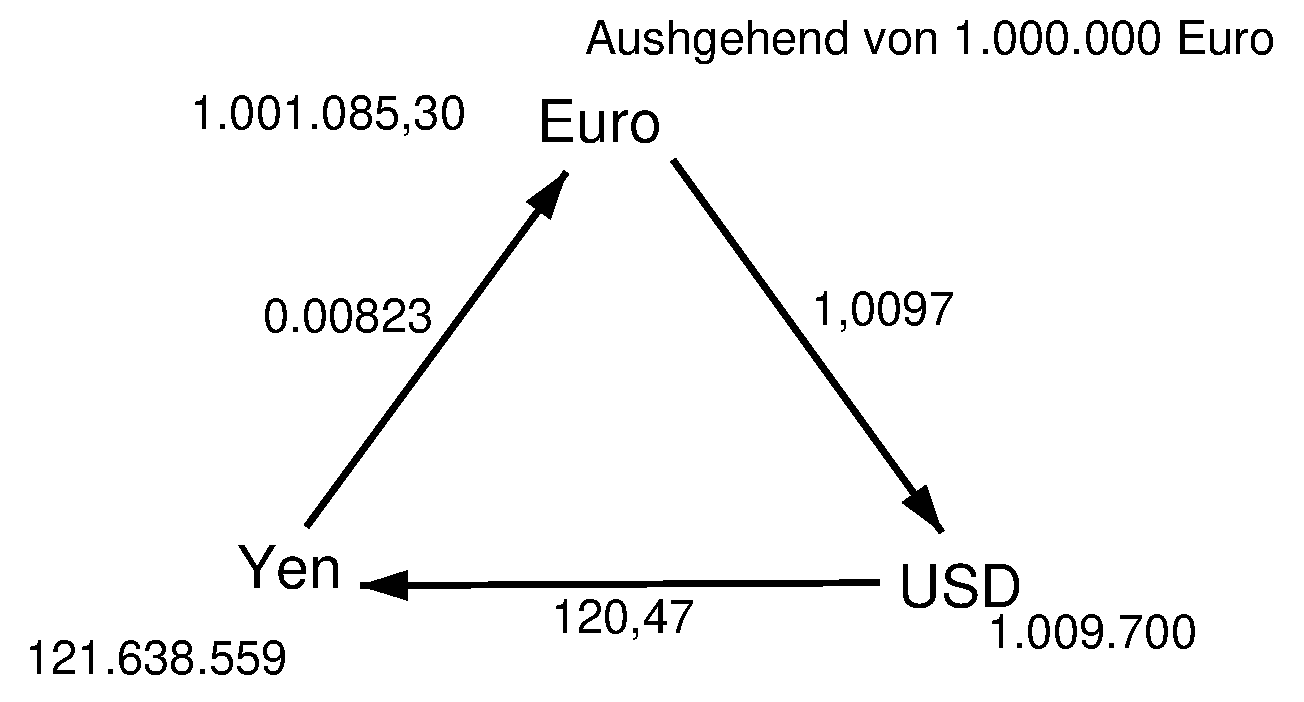
\includegraphics[width=8cm]{bilder/2-2Arbitrage}\\
Arbitrage-Möglichkeiten mit den Kursen vom 18.11.2002
\end{tabular}

Gesucht sind also Folgen $v_{0}, v_{1}, \ldots, v_{k} = v_{0}$ mit:
\[\prod^{k}_{i=1} r_{v_{i-1} v_{i}} > 1\] 

Kosten: $c_{u v} = -\log r_{u v}$

Gewinn falls $\sum_{i=1}^{k} \log r_{v-1v_{i}} = - \log \prod_{i=1}^{k}
r_{v_{i-1}v_{i}} < 0$

\begin{lemma} \label{Ford1}
Hat $(G,c)$ keinen negativen Kreis, so gilt nach jeder Iteration von Fords
Algorithmus:
\begin{enumerate}
\item Ist $y_{v} \not= \infty$ so ist $y_{v}$ Kosten eines einfachen 
$(r,v)$-Weges 
\item Ist $p(v) \not = -1$ so definiert $p$ einen einfachen $(r,v)$-Weg mit
Kosten höchstens $y_{v}$ 
\end{enumerate}
\end{lemma}

Beweis: 
\begin{enumerate}
\item Sei $y_{v}^{j}$ der Wert $y_{v}$ nach $j$ Iterationen.\\
$y_{v}^{j}\not= \infty \rightarrow  y_{v}^{j}$ Kosten eines
$(r,v)$-Weges $P$.\\
Annahme: $P$ ist nicht einfach $\Rightarrow \exists$ Folge $v_{0}, v_{1},
\ldots, v_{k}$,  $v_{k}= v_{0}$\\
Iterationszahlen $q_{0} < q_{1} < \ldots < q_{k}$ mit $y_{v-1}^{q_{i-1}} +
c_{v_{i-1}v_{i}} = y_{v_{i}}^{q_{i}}$\\
und Kosten des geschlossenen Weges:
\[\begin{array}{rcl}
\displaystyle \sum_{i=1}^{k} c_{v_{i-1}v_{i}} &=& \displaystyle \sum_{i=1}^{k} 
(y_{v_{i}}^{q_{i}} - y_{v_{i-1}}^{q_{i-1}})\\
&=& y_{v_{k}}^{q_{k}} - y_{v_{0}}^{q_{0}} < 0
\end{array}\]
$y_{v_{k}}$ wurde in Iteration $q_{k}$ erniedrigt. Also haben wir einen
negativen Kreis und damit Widerspruch. 
\item Annahme $P$ ist nicht einfach\\
$\Rightarrow \exists v_{0}, v_{1}, \ldots , v_{k}$, $v_{k}= v_{0}$\\
$p(v_{i})=v_{i-1}$  \hspace{3mm} $(1\leqq i \leqq k)$\\
Die Kosten des geschlossenen Weges sind $\leqq 0$, da $c_{p(v)v}  \leqq
y_{v} - y_{p(v)}$\\
Die letzte Änderung ergibt: $p(v)$ mit Verkleinerung von $y_{p}(v_{i})$
$\Rightarrow$ "`$<$"'\\
$\Rightarrow$ negativer Kreis, Widerspruch  
\end{enumerate}

Die Kosten sind höchstens $y_{v}$:
Es gebe einen einfachen $(r,v)$-Weg und sei $v_{0}, e_{1}, v_{1}, \ldots,
e_{k}, v_{k}$ mit $v_{0} = r$, $v_{k}=v$, $p(v_{i}) = v_{i-1}, \; \; \; 
(1 \leqq i \leqq k)$\\
Kosten $\displaystyle \sum_{i=1}^{k} c_{v_{i-1}v_{i}} \leqq  \sum_{i=1}^{k}
(y_{v_{i}} - y_{v_{i-1}}) = y_{v} - y_{r} = y_{v}$ q.e.d.

\begin{satz}
Hat $(G,c)$ keinen negativen Kreis, so terminiert Fords Algorithmus nach
endlich vielen Schritten mit einem korrekten Ergebnis
\end{satz}

Beweis:\\
$\exists$ nur endlich viele einfache gerichtete Wege in $G$.\\
Lemma \ref{Ford1} $\Rightarrow$ Es gibt nur endlich viele mögliche Werte
für die $y_{v}$. In jedem Schritt wird ein $y_{v}$ erniedrigt und keines
erhöht $\rightarrow$ endlich viele Schritte.

Bei Terminierung definiert $p$ einfache $(r,v)$-gerichtete Wege für alle
$v \in V$ mit Kosten höchstens $y_{v}$.\\
Lemma \ref{Potential} $\Rightarrow$ Es gibt keine kürzere
$(r,v)$-gerichtete Wege.

\begin{satz} \label{Potential2}
$(G,c)$ hat ein zulässiges Potential genau dann, wenn es keinen negativen
Kreis gibt.
\end{satz}

Beweis:\\
"`$\Rightarrow$"' negativer Kreis $\Rightarrow$ kein zulässiges Potential

"`$\Leftarrow$"' $(G,c)$ habe keinen negativen Kreis:\\
Man konstruiere folgenden Graphen $(G',c')$:

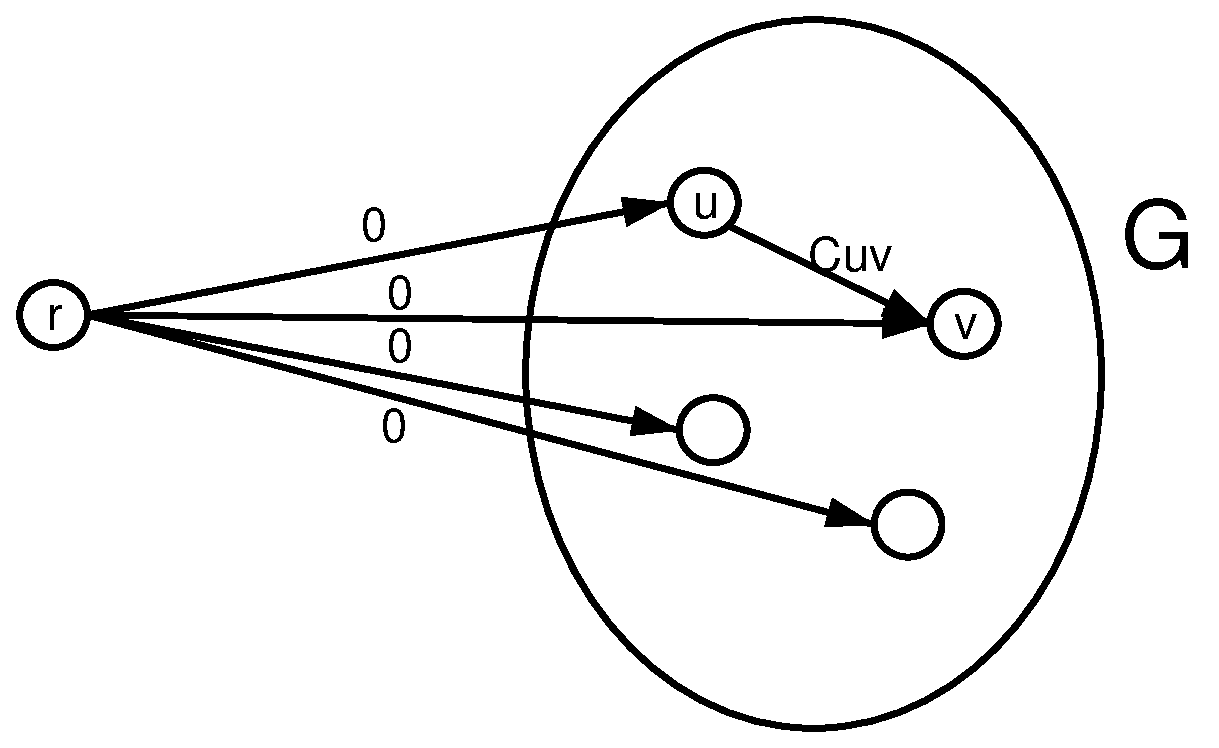
\includegraphics[width=9cm]{bilder/2-2NegatKreis}

$r$ ist jeweils mit allen Knoten von $G$ durch gerichtete Kanten des
Gewichtes 0 verbunden. Damit hat $(G',c')$ keinen negativen Kreis.
Anwendung von Fords Algorithmus auf $(G',c')$ gibt zulässiges Potential für 
$(G',c')$. Diese ist auch zulässiges Potential für $(G,c)$. q.e.d.

Satz \ref{Potential2} Gilt auch ohne Annahme der Existenz von
$(r,v)$-Wegen.\\
Problem: nicht einfache beliebig kurze $(r,v)$-gerichtete Wege.\\
Die Suche nach einfachen (r,v)-Wegen (endlich viele!) ist jedoch
NP-schwierig.

\begin{satz}
Falls $c_{e} \in \ZZ$ für alle $e \in E$:
\[ c = 2 \max_{e \in E} | c_{e} | + 1 \]
und $(G,c)$  hat keinen negativen Kreis so terminiert Fords Algorithmus
nach höchstens $c n^{2}$ Iterationen
\end{satz}
Beweis: Übungsaufgabe

\subsection{Zulässige Potentiale und lineare Optimierung}

\begin{satz} 

Sei $G$ ein gerichteter Graph, $r,s \in V$, $c \in \RR^{E}$\\
Falls für alle $v \in V$ ein kürzester  $(r,v)$-Weg existiert, so gilt:\\
\[\begin{array}{cl}
&\min \left\{c(P) | P \mbox{ ist $(r,s)$ gerichteter Weg} \right\}\\
=& \max \left\{ y_{s} | y \mbox{ ist ein zulässiges Potential}\right\}
\end{array}\]
\end{satz}
Beweis: Analyse von Fords Algorithmus

Als duales LP formuliert erhält man (ohne Bedingung $y_{r}=0$):
\[\begin{array}{rcl}
\mbox{(DLPKW)} \hspace{7mm} \max y_{s} -y_{r}\\
y_{w} - y_{v} \leqq c_{v w} \; \; \; \forall v,w \in E
\end{array}\]

Für das LP definieren wir:\\
Sei $b_{v} = \left\{ \begin{array}{l} 1 \mbox{ falls } v =s\\
-1 \mbox{ falls } r =v\\
0 \mbox{ sonst}\\
\end{array} \right.$

\[\begin{array}{rcl}
\mbox{(LPKW)} \hspace{7mm} \min \displaystyle \sum_{e \in E} c_{e} x_{e}\\
\displaystyle \sum_{w \in V, \; \; v w \in E} x_{w v} -  \sum_{w \in V, \;
\; w v \in E} x_{v w} &=& b_{v} \; \; \; \forall v \in V\\
x_{v w} &\geqq & 0  \; \; \; \forall v w \in E
\end{array}\]

Jedem $(r,s)$-gerichteten Weg $P$ entspricht eine zulässige Lösung für
(LPKW) mit Wert $c(P)$.
$x_{e}^{P} = $ Anzahl des Vorkommens von $e$ in $P$. ($\in \{0,1\}$ falls
$P$ einfach ist).

\subsubsection{Verhalten des Simplexalgorithmus beim LPKW}

Gegeben sei folgender Graph:

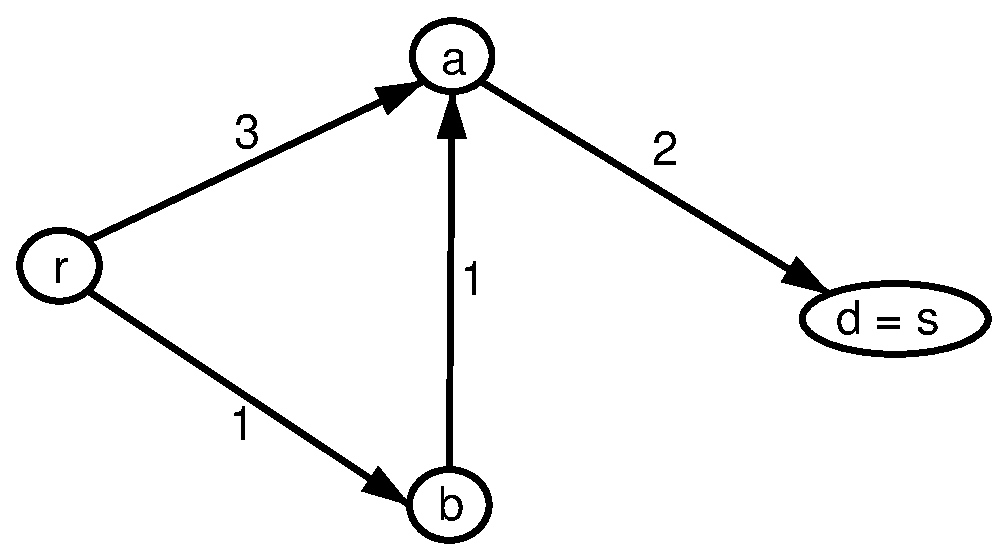
\includegraphics[width=6cm]{bilder/2-2SimplLPKW}

Dann ergibt sich folgender Aufbau:

A \hspace{3mm}
\begin{tabular}{c|rrrr|}
\multicolumn{1}{c}{\mbox}&r a&r b& b a&\multicolumn{1}{r}{ad}\\ \cline{2-5}
r&-1&-1&&\\
a&1&&1&-1\\
b&&1&-1&\\
d&&&&1\\
\cline{2-5}
\end{tabular} $=$ \begin{tabular}{|r|}
\multicolumn{1}{c}{b}\\\hline-1\\\mbox{}\\\mbox{}\\1\\\hline
\end{tabular}
\hspace{4mm}$\begin{array}{rcl}
\mbox{(LKWP)} \hspace{3mm} \min c^{T}x\\
A x &=& b\\
x &\geqq& 0
\end{array}$

c\hspace{12mm}\begin{tabular}{|rrrr|}
\hline 3&1&1&2\\ \hline
\end{tabular}

Der Simplexalgorithmus betrachtet nun eine Folge von Basislösungen wobei
eine Basis einer "`max. linear unabh. Kantenteilmenge"' entspricht. Es ist
also eine "`Spaltenbasis"' von A.

In jeder Iteration hat man eine Basis $B$ und $x,y$ mit $x_{e} = 0 \; \; \forall
e \not\in B$.
\[y_{w} - y_{v} = c_{v w} \forall v w \in B\]

\begin{satz} \label{Spaltenb-Baum}
Sei $G$ ein zusammenhängender gerichteter Graph, $A$ die Knoten-Kanten
Inzidenzmatrix.

$A_{\cdot J}, \; \; J \subseteq E$ ist eine Spaltenbasis von $A$ genau dann
wenn $J$ die Kantenmenge eines Aufspannenden Baumes in $G$ ist.
\end{satz}

Beweis: Übungsaufgabe

Baum $T_{1}$

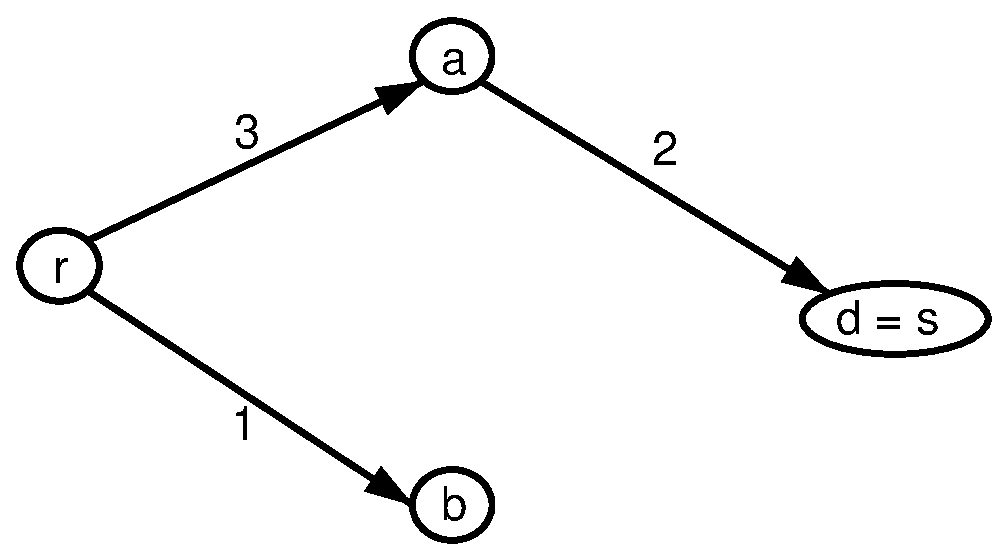
\includegraphics[width=6cm]{bilder/2-2SimplLPKW2}

Ein Basiswechsel Beispiel.

B \hspace{3mm}
\begin{tabular}{c|rrr|}
\multicolumn{1}{c}{\mbox}&r a&r b&\multicolumn{1}{r}{ad}\\ \cline{2-4}
r&-1&-1&\\
a&1&&-1\\
b&&1&\\
d&&&1\\
\cline{2-4}
\end{tabular} $=$ \begin{tabular}{|r|}
\multicolumn{1}{c}{y}\\\hline0\\3\\1\\5\\\hline
\end{tabular}

c\hspace{12mm}\begin{tabular}{|rrr|}
\hline 3&1&2\\ \hline
\end{tabular}

reduzierte Kosten: $c_{b a} - y^{T}A_{\cdot b a} = 1 -2 = -1 < 0$

$\rightarrow$ $b a$ geht in die Basis, $r a$ raus (hat die Spitze am selben
Punkt).

Baum $T_{2}$

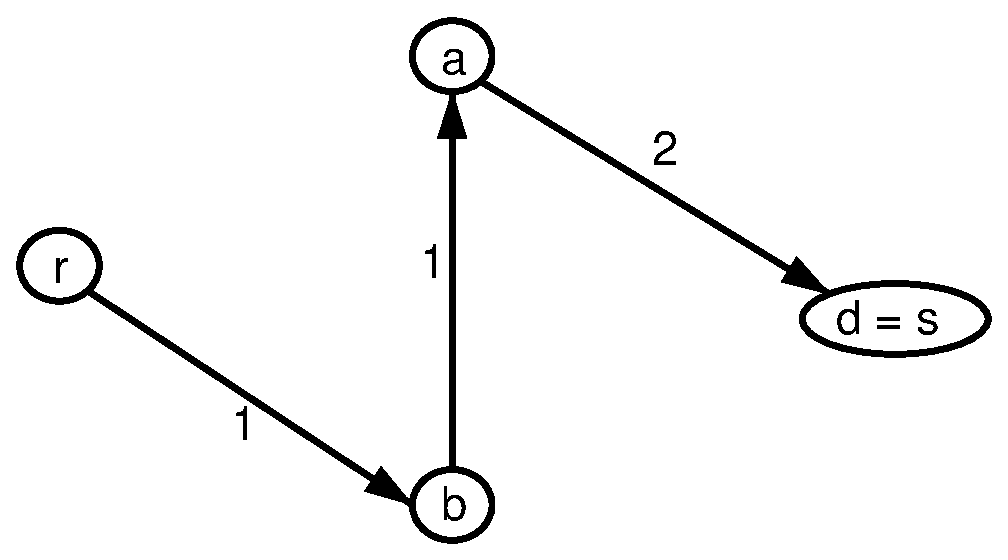
\includegraphics[width=6cm]{bilder/2-2SimplLPKW3}

B \hspace{3mm}
\begin{tabular}{c|rrr|}
\multicolumn{1}{c}{\mbox}&r a&b a&\multicolumn{1}{r}{ad}\\ \cline{2-4}
r&-1&&\\
a&&1&-1\\
b&1&-1&\\
d&&&1\\
\cline{2-4}
\end{tabular} $=$ \begin{tabular}{|r|}
\multicolumn{1}{c}{y}\\\hline0\\2\\1\\4\\\hline
\end{tabular}

c\hspace{12mm}\begin{tabular}{|rrr|}
\hline 3&1&2\\ \hline
\end{tabular}

reduzierte Kosten: $3-2 = 1 > 0$

Die Gleichungen $y_{w} - y_{v} = c_{v w} \forall v w \in B$ gelten in Fords
Algorithmus nicht immer, d.h. jede Iteration dieses speziellen Simplex
Verfahrens entspricht einer Folge von Iterationen in Fords Algorithmus
(Änderung des Baumes gefolgt von $y$-Änderungen bei gleichem Baum. 

\subsection{Varianten des Ford Algorithmus}

Korrekturschritte in konstanter Zeit. Laufzeit abhängig von der
Reihenfolge  $S= <f_{1}, f_{2}, \ldots, f_{e}>$ der gewählten Kanten. Bei
schlechter Wahl erhält man eine Laufzeit von $\Theta(2^{|E|})$ (Übungen)

Ein $(r,v)$-Weg $P= \; \; r=v_{0}, e_{1}, v_{1}, \ldots, c_{k}, v_{k} = v$
ist in $S$ eingebettet falls $e_{1}, e_{2},\ldots_{k}$ eine geordnete
Subsequenz von $S$ ist.

\begin{lemma} \label{Ford2}
Wenn Fords Algorithmus die Sequenz $S$ benutzt, so gilt für jedes $v \in V$
und jeden $(r,v)$-Weg der in $S$ eingebettet ist $y_{v} \leqq c(P)$
\end{lemma}

Beweis: Sei $P = \; \;  \underbrace{v_{0}}_{\mbox{\scriptsize$=r$}}, 
e_{1}, v_{1}, \ldots, c_{k}, \underbrace {v_{k}}_{\mbox{\scriptsize $= v$}}$\\
Nach erster Iteration mit $e_{1}: y_{v_{1}} \leqq y_{r} + c_{e_{1}}$\\
Nach zweiter Iteration mit $e_{2}: y_{v_{2}} \leqq y_{v_{1}} + c_{e_{1}}+ 
c_{e_{2}}$\\
Nach dritter Iteration mit$\begin{array}[t]{rcl}e_{k}: y_{v} = y_{v_{k}} &\leqq & y_{v_{k-1}} + c_{e_{k}}\\
&\leqq & \displaystyle \sum_{i=1}^{k} c_{e_{i}} = c(P). \hspace{3mm}
\mbox{q.e.d}\end{array}$

Also suchen wir $S$ mit kürzesten eingebetteten $(r,v)$-Wegen für alle $v
\in V$ $S$
"`kurz"' da die Laufzeit proportional zur Länge.

\subsubsection{Ford-Bellmann-Algorithmus}

Jeder einfache gerichtete Weg in $G$ ist eingebettet in
$<s_{1},s_{2},s_{3},
\ldots, s_{n-1} >$ mit $s_{i} =$ irgendeine Permutation von $E= \{ e_{1},
e_{2}, \ldots, e_{m}\}$

\begin{algorithmic}
\STATE Initialisiere $y, \; p$;
\STATE $i=0$;
\WHILE{($i < n$ und $y$ kein zulässiges Potential)}
\STATE i := i+1;
\FOR{ $e=e_{1}$ to $e_{m}$}
\STATE $v=t(e)$; $w=h(e)$;
\IF{$(y_{v} + c_{v w} < y_{w})$}
\STATE $y_{w} := y_{v} + c_{v w}$; $p_{w} := v$
\ENDIF
\ENDFOR
\ENDWHILE
\IF{$(i < n)$} 
\STATE "`Kürzester Weg gefunden"'
\ELSE 
\STATE STOP "`es existiert ein negativer Kreis"'
\ENDIF
\end{algorithmic}


\begin{satz}
Der Ford-Bellmann Algorithmus ist korrekt und hat Laufzeit $O(n m)$.
\end{satz}

Beweis: Korrektheit wg. Lemma \ref{Ford2}, Laufzeit offensichtlich.

Verbesserungen der Laufzeit sind nur bei speziellen Annahmen über $G$ und
$c$ möglich. Vorgestellt werden nun Verbesserungen in der Praxis:

\paragraph{Vorwärts-Stern-Datenstruktur}
\mbox{} 

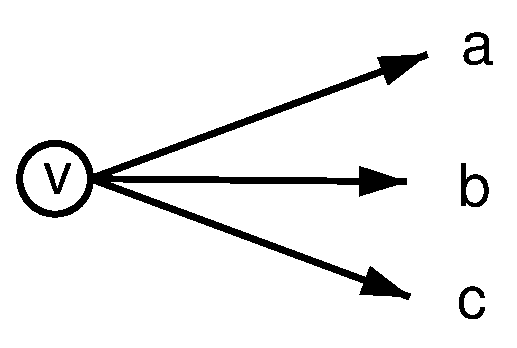
\includegraphics[width=4cm]{bilder/2-2VorwaertsStern} $L(v)=<a,b,c>$

Weiterhin benötigen wir:\\
$Q= <f_{1}, f_{2}, \ldots, f_{e}>$ Schlange (Queue) von Kunden.\\
$v \Leftarrow Q$ ergibt $v=q_{1},\; \;  Q = <f_{2}, f_{3}, \ldots,
f_{e}>$\\
$Q \Leftarrow v$ ergibt $Q= <f_{1}, f_{2}, \ldots, f_{e}, v>$\\
Zusätzlich Inzidenzvektor: isinQ Q[v]\\
Anzahl der Knoten in Q: numQ 

dies erlaubt delete, append $Q \stackrel{?}{=} \varnothing, \; \; v \stackrel{?}{\in} Q$ in konst.
Zeit (keine Negativen Kreise).

\begin{algorithmic}
\STATE Initialisiere $y,\;p$;
\STATE $Q:= <v>$;
\WHILE{$(Q \not= \varnothing)$}
\STATE $v \Leftarrow Q$;\\
\FORALL{$\left(w \in L(v)\right)$}
\IF{$(y_{v} + c_{v w} < y_{w})$}
\STATE $y_{w} := y_{v} + c_{v w}$; $p_{w} := v$ \}\\
\IF{$(w \not\in Q)$}
\STATE $Q \Leftarrow w$;
\ENDIF
\ENDIF
\ENDFOR
\ENDWHILE
\end{algorithmic}

\paragraph{Azyklische Graphen}
\mbox{}\\
Keine gerichteten Kreise, insbesondere keine negativen Kreise. Kompatible
Knoten Sequenz $<v_{1}, v_{2}, \ldots, v_{n}>$ für alle Knoten $v_{i},
v_{j} \in E$ gilt: $i < j$ kann in Zeit $O(m)$ gefunden werden (Topologische
Sortierung, siehe Übungsaufgabe 20).

OBdA: sei $r=v_{1}$
\[ r=v_{i} \; \Rightarrow \; v_{j} \; \; \; (j < i) \mbox{ nicht erreichbar} \]
wie oben, aber:

\begin{algorithmic}
\STATE $\vdots$
\FOR{$i=1$ to $n$}
\FORALL{$\left(w \in L(v_{i})\right)$}
\STATE (jeder Pfad ist eingebettet)
\IF{$(y_{v} + c_{v w} < y_{w})$}
\STATE $y_{w} := y_{v} + c_{v w}$; $p_{w} := v$ 
\ENDIF
\ENDFOR
\ENDFOR
\end{algorithmic}

\begin{satz}
In azyklischen Graphen kann das kürzeste Wege Problem in Zeit $O(m)$
gelöst werden
\end{satz}

Nicht negative Kosten:
\[ c_{e} \geqq 0 \; \; \forall e \in E\]
Wie vorhin, aber Knotensequenz dynamisch bestimmt nach $v_{1}, v_{2},
\ldots, v_{i}$.\\
Wähle $v_{i+1} = v \in \{v_{1}, v_{2}, \ldots,v_{i}\}$ mit minimalem
$y_{v}$.

\begin{lemma} \label{UvorV}
Für alle $w \in V$ sei $y'_{w}$ der Wert von $y_{w}$ wenn $w$ gewählt wird.
Wird $u$ vor $v$ gewählt. So gilt $y'_{u} \leqq y'_{v}$.
\end{lemma}

Beweis: Annahme $y'_{v} < y'_{u}$ und $v$ ist der erste Knoten bei dem das
passiert.\\
Als $u$ gewählt wurde galt: $y'_{u} = y_{u} \leqq y_{v}$. Nach Wahl von $u$
und vor Wahl von $v$ wurde $y_{v} < y'_{u}$, sagen wir das letzte Mal
bei Wahl von $w$
\[v_{1}, v_{2}, \ldots, u, \ldots, w, \ldots,v,\ldots\]
Also fand bei $w$ die letzte Erniedrigung von $y_{v}$ statt. Zu diesem
Zeitpunkt wurde gesetzt:
\[y_{v} := y'_{w} + c_{w v}\]
Aber $\left. \begin{array}{rcl}
y'_{w} &>& y'_{u} \hspace{3mm} \mbox{(erster Fehler bei $v$)}\\
c_{v w} &\geqq& 0
\end{array}
\right\} y'_{v} \geqq y'_{u} \hspace{4mm} \lightning$

\subsubsection{Dijkstras Algorithmus}

\begin{algorithmic}
\STATE Initialisiere $y$, $p$;
\STATE $S := V$
\WHILE{$(S \not= \varnothing)$}
\STATE wähle $v \in S$ mit $y_{v}$ minimal
\STATE entferne $v$ aus $S$;
\STATE Bearbeite Vorwärtsstern von $v$ (aber nur Kanten mit $vw$ mit $w \in
S$!)
\ENDWHILE
\end{algorithmic}


\begin{satz}
Falls $c_{e} \geqq 0 \; \; \forall e \in E$, so ist Dijkstras Algorithmus
korrekt und läuft in $O(n^{2})$
\end{satz}

Beweis:\\
Am Ende gilt ($\ast$) $y_{v} + c_{v w} \geqq y_{w} \; \; \forall \; v w \in
E$

Annahme: ($\ast$) gilt nicht\\
($\ast$) galt nach Bearbeitung von Knoten v $\Rightarrow y_{v}$ wurde
später erniedrigt, etwa als $q$ bearbeitet wurde. \\
$\Rightarrow y_{v} = \underbrace{y'_{q}}_{\geqq y'_{v}} + \underbrace{c_{q v}}_{\geqq 0}  \geqq y'_{v}$ 
also nicht erniedrigt $\lightning$\\
denn wenn q nach v bearbeitet wurde $\stackrel{\mbox{\scriptsize Lemma
\ref{UvorV}}}{\Rightarrow} y'_{q} \geqq y'_{v}$\\
$w \not \in S$: $y_{v} \geqq y_{w} \stackrel{\mbox{\scriptsize Lemma
\ref{UvorV}}}{\Rightarrow} y_{v} + \underbrace{c_{v w}}_{\geqq 0} \geqq
y_{w v}$ also hier kein Test nötig. 

Laufzeit $O(m)$ für Vorwärtsstern plus die Zeit zum Finden von $v$ mit
minimalem $y_{v}$. Naiv implementiert erhält man damit eine Laufzeit von
$O(n^{2})$

Aus der Informatik I. Für Dünne Graphen mit Heaps $O(m \log n)$. Noch besser
geht es mit Fibonacci Heaps (Wer hat die Fibonacci Beweise nicht geliebt?):
$O(n \log n + m)$.

Wie dem auch sei, sei $S(n,m)$ die Zeit, die benötigt wird.

Beobachtung:\\
Kennt man ein zulässiges Potential $y$ so kann man den Kostenvektor $c$
nach $c' \geqq 0$ transformieren: $c'_{v w} = c_{v w} + y_{v} - y_{w} (\geqq 0)$ 
denn  $\forall (r,s)$-Wege $P$: sind die Kosten: 
\[c'(P) = c(P) + y_{r} - y_{s}\]  
Anwendung: Kürzeste $(r,v)$-Wege für alle Paare (r,v). Allgemein beste
Methode: n mal wie gehabt.\\
Zeit $O(n \cdot S(n,m))$, wenn $c \geqq 0$, also $O(n^{2}m)$ im allgemeinen
Fall.

Verbesserung von $O(n^{2}m)$: Wenn Ford Bellman einmal ausgeführt ist
liefert er uns ein zulässiges Potential für jeden Punkt.
\[\left. \begin{array}{l}
\mbox{Transformation s.o.}\\
\mbox{$(n-1)$ mal Dijkstra}\end{array} \right\} \mbox{zusammen } O(n \cdot
S(n,m))
\]

\subsubsection{Einheitskosten und Breitensuche}

Finde $(r,v)$-Wege mit minimaler Kantenzahl.

\begin{lemma} \label{ErsterW}
Falls $c_{e} = 1$ für alle $e \in E$, so ist der erste endliche Wert für
$y_{v}$ auch der endgültige. Wird $y_{v}$ vor $y_{w}$ zugewiesen, so gilt
$y_{v} \leqq y_{w}$.
\end{lemma}

Beweis: klar für $v=r$. Sei $v \not=r$ und $v$ später gewählt als Knoten
$u \Rightarrow y_{v} \geqq y_{u}$ (Lemma \ref{UvorV}).\\
zu endgültig: Erster endliche Wert für $y_{v}$ wird gesetzt zu $y_{w+1}$
[Knoten $w$ wird vor $v$ gewählt]


Behauptung $y_{v}$ wird nicht mehr geändert \\
Annahme: bei  Wahl eines anderen Knotens z.B. $q$ wird $y_{v}$ erniedrigt
zu $y'_{v}$.\\
Situation: $\ldots w \ldots v \ldots q$\\
$q$ wird nach $w$ gewählt $ \Rightarrow y_{q} \geqq y_{w}$\\
$y'_{v} = y_{q} + 1 \geqq y_{w} + 1 = y_{v} \; \; \; \lightning$ zu
erniedrigt.

\begin{satz}
Bei Einheitskosten kann Dijkstras Algorithmus mit Laufzeit $O(m)$
implementiert werden.
\end{satz}
Beweis: Wegen Lemma \ref{ErsterW} kann man den nächsten Knoten aus einer
Schlange wählen ($y_{w}$ sind überflüssig).

Dieser Algorithmus heißt auch Breitensuche.

\begin{algorithmic}
\STATE Initialisiere p;
\STATE $Q = <r>;$\\
\WHILE{$(Q \not= \varnothing)$}
\STATE $v \Leftarrow Q$;
\FORALL{$(w \in L(v))$}
\IF{$(p(w) = -1)$}
\STATE $Q \Leftarrow w$;
\STATE $p(w) = v$;
\ENDIF
\ENDFOR
\ENDWHILE
\end{algorithmic}



